%%%%%%%%%%%%%%%%%%%%%%%%%%%%%%%%%%%%

\section{3.4. Distribuição binomial}

%%%%%%%%%%%%%%%%%%%%%%%%%%%%%%%%%%%%

\subsection{A distribuição binomial}

%%%%%%%%%%%%%%%%%%%%%%%%%%%%%%%%%%%%

\begin{frame}
\frametitle{Exemplo}
\justifying
\dq{Suponha que selecionamos aleatoriamente quatro indivíduos para participar desta experiência. Qual é a probabilidade de que exatamente um deles se recuse a administrar o choque?}
\pause
\justifying
Vamos chamar essas pessoas de Allen (A), Bretanha (B), Caroline (C) e Damian (D). Cada um dos quatro cenários abaixo irá satisfazer a condição de "exatamente 1 deles se recusa a administrar o choque":\\
\vspace{0.25cm}
\pause
\begin{changemargin}{+1.5cm}{+0cm}
{\footnotesize
\begin{enumerate}

\item[Cenário 1:] $\slot{0.35}{\text{(A) \orange{recusa}}} \times \slot{0.65}{\text{(B) choque}} \times \slot{0.65}{\text{(C) choque}} \times \slot{0.65}{\text{(D) choque}} = 0.0961$
\pause
\item[Cenário 2:] $\slot{0.65}{\text{(A) choque}} \times \slot{0.35}{\text{(B) \orange{recusa}}}\times \slot{0.65}{\text{(C) choque}} \times \slot{0.65}{\text{(D) choque}} = 0.0961$
\pause
\item[Cenário 3:] $\slot{0.65}{\text{(A) choque}} \times \slot{0.65}{\text{(B) choque}} \times \slot{0.35}{\text{(C) \orange{recusa}}}\times \slot{0.65}{\text{(D) choque}} = 0.0961$
\pause
\end{enumerate}
}
\end{changemargin}
\end{frame}
%%%%%%%%%%%%%%%%%%%%%%%%%%%%%%%%%%%%

\begin{frame}
\frametitle{Exemplo}

\begin{changemargin}{+1.5cm}{+0cm}
{\footnotesize
\begin{enumerate}

\item[Cenário 4:] $\slot{0.65}{\text{(A) choque}} \times \slot{0.65}{\text{(B) choque}} \times \slot{0.65}{\text{(C) choque}} \times \slot{0.35}{\text{(D) \orange{recusa}}} = 0.0961$
\end{enumerate}
}
\end{changemargin}
\pause
\justifying
A probabilidade de exatamente 1 de 4 pessoas se recusarem a administrar o choque é a soma de todas essas probabilidades.
\[ 0.0961+ 0.0961 + 0.0961 + 0.0961 = 4 \times 0.0961 = 0.3844 \]

\end{frame}

%%%%%%%%%%%%%%%%%%%%%%%%%%%%%%%%%%%%

\begin{frame}
\frametitle{Distribuição binomial}
\justifying
A pergunta anterior pedia a probabilidade de um determinado número de sucessos, \mathhl{k}, em um determinado número de tentativas, \mathhl{n}, ($ k = 1 $ sucesso em $ n = 4 $ tentativas). Essa probabilidade é calculada como
\[ \#~ de ~ cenarios \times P(unico ~ cenario) \]

\pause

\begin{itemize}
\justifying
\item $\#~ de ~ cenarios$: há um modo mais direto de descobrir isso, discutiremos em breve...

\pause
\justifying
\item $P(unico ~ cenario) = p^k~(1-p)^{(n-k)}$ \\
\justifying
{\scriptsize{ onde p é a probabilidade de sucesso elevada a quantidade de sucessos k e (p-1) é a probabilidade de fracassos elevada a quantidade de fracassos (n-k)}}

\end{itemize}

\pause
\justifying
A \hl{Distribuição binomial} descreve a probabilidade de ter exatamente $ k $ sucessos em $ n $ tentativas de Bernoulli independentes com probabilidade de sucesso $p$.

\end{frame}

%%%%%%%%%%%%%%%%%%%%%%%%%%%%%%%%%%%%

\begin{frame}
\frametitle{Contando o \# de cenários}
\justifying
Anteriormente escrevemos todos os cenários possíveis que se encaixam na condição de exatamente uma pessoa se recusando a administrar o choque. Se $ n $ for maior e/ou $ k $ for diferente de 1, por exemplo, $ n = 9 $ e $ k = 2 $:

\pause

\begin{center}
\begin{tabular}{c}
\orange{R}\orange{R}SSSSSSS \\ 
\pause
S\orange{R}\orange{R}SSSSSS \\
\pause
SS\orange{R}\orange{R}SSSSS \\
$\cdots$ \\
SS\orange{R}SS\orange{R}SSS \\
$\cdots$ \\
SSSSSSS\orange{R}\orange{R} \\
\end{tabular}
\end{center}
\justifying
Escrever todos os cenários possíveis seria extremamente tedioso e propenso a erros.

\end{frame}

%%%%%%%%%%%%%%%%%%%%%%%%%%%%%%%%%%%%

\begin{frame}[fragile]
\frametitle{Calculando o \# de cenários}
\justifying
\formula{Fórmula da combinação}
{
\justifying
A \hl{fórmula da combinação} é útil para calcular o número de maneiras de obter $ k $ sucessos em $ n $ tentativas.
\[ {n \choose k} = \frac{n!}{k! (n - k)!} \]
}

\pause

\begin{itemize}

\item $k = 1$, $n = 4$: ${4 \choose 1} = \frac{4!}{1! (4 - 1)!} = \frac{4 \times 3 \times 2 \times 1}{1 \times (3 \times 2 \times 1)} = 4$

\pause

\item $k = 2$, $n = 9$: ${9 \choose 2} = \frac{9!}{2! (9 - 1)!} = \frac{9 \times 8 \times 7!}{2 \times 1 \times 7!} = \frac{72}{2} = 36$

\end{itemize}

\vfill
\justifying
\Note{Você também pode usar R para esses cálculos:}
\begin{beamerboxesrounded}[shadow = true, lower = code body]{}
{\small
\begin{verbatim}
> choose(9,2)
[1] 36
\end{verbatim}
}
\end{beamerboxesrounded}

\end{frame}

%%%%%%%%%%%%%%%%%%%%%%%%%%%%%%%%%%%

\begin{frame}[fragile]
\frametitle{Propriedades da função escolher}
\justifying
\pq{Qual das seguintes afirmações é falsa?}

\begin{enumerate}[(a)]
\justifying
\item Existem $ n $ maneiras de obter 1 sucesso em $ n $ tentativas, ${n \choose 1} = n$.
\justifying
\item Existe apenas uma maneira de obter $ n $ sucessos em $ n $ tentativas, ${n \choose n} = 1$.
\justifying
\item Existe apenas uma maneira de obter fracassos de $ n $ em $ n $ tentativas, ${n \choose 0} = 1$.
\justifying
\solnMult{Existem $ n-1 $ maneiras de obter $ n-1 $ sucessos em $ n $ tentativas, ${n \choose n-1} = n-1$.}
\end{enumerate}

\end{frame}

%%%%%%%%%%%%%%%%%%%%%%%%%%%%%%%%%%%

\begin{frame}
\frametitle{Distribuição binomial (cont.)}
\justifying
\formula{Probabilidades Binomiais}
{
\justifying
Se $ p $ representa probabilidade de sucesso, $ (1-p) $ representa probabilidade de fracasso, $ n $ representa número de tentativas independentes e $ k $ representa número de sucessos
\[P(k~sucessos~em~n~tentativas) = {n \choose k}~p^k~(1-p)^{(n-k)} \]
} 


\end{frame}

%%%%%%%%%%%%%%%%%%%%%%%%%%%%%%%%%%%

\begin{frame}
\frametitle{Prática}
\justifying
\pq{Qual das seguintes opções não é uma condição que precisa ser atendida para que a distribuição binomial seja aplicável?}

\begin{enumerate}[(a)]
\justifying
\item os ensaios devem ser independentes.
\justifying
\item o número de tentativas, $ n $, deve ser fixo.
\justifying
\item cada resultado de uma tentativa deve ser classificado como \textit{sucesso} ou \textit{fracasso}.
\justifying
\item o número de sucessos desejados, $ k $, deve ser maior que o número de tentativas.
\justifying
\item a probabilidade de sucesso, $ p $, deve ser a mesma para cada tentativa.
\end{enumerate}

\end{frame}

%%%%%%%%%%%%%%%%%%%%%%%%%%%%%%%%%%%

\begin{frame}
\frametitle{Prática}
\justifying
\pq{Uma pesquisa de 2012 do Gallup sugere que 26,2 \% dos americanos são obesos. Entre uma amostra aleatória de 10 americanos, qual é a probabilidade de exatamente 8 serem obesos?}

\begin{enumerate}[(a)]
\item muito alta
\solnMult{muito baixa}
\end{enumerate}

\vfill

\ct{Gallup: \webURL{http://www.gallup.com/poll/160061/obesity-rate-stable-2012.aspx}, Janeiro 23, 2013.} 

\end{frame}

%%%%%%%%%%%%%%%%%%%%%%%%%%%%%%%%%%%%

\begin{frame}
\frametitle{Prática}
\justifying
\pq{Uma pesquisa de 2012 do Gallup sugere que 26,2 \% dos americanos são obesos. Entre uma amostra aleatória de 10 americanos, qual é a probabilidade de exatamente 8 serem obesos?}

\begin{enumerate}[(a)]
\item $0.262^8 \times 0.738^2$
\item ${8 \choose 10} \times 0.262^8 \times 0.738^2$
\solnMult{${10 \choose 8} \times 0.262^8 \times 0.738^2$} \soln{\orange{\only<2>{$ = 45 \times  0.262^8 \times 0.738^2 = 0.0005$}}}
\item ${10 \choose 8} \times 0.262^2 \times 0.738^8$
\end{enumerate}



\end{frame}

%%%%%%%%%%%%%%%%%%%%%%%%%%%%%%%%%%%

\begin{frame}
\frametitle{O problema do aniversário}
\justifying
\dq{Qual é a probabilidade de que 2 pessoas escolhidas aleatoriamente façam aniversário no mesmo dia?}

\pause
\justifying
Muito baixa, $\frac{1}{365} \approx 0.0027$.

\pause
\justifying
\dq{Qual é a probabilidade de que pelo menos 2 pessoas de 366 pessoas façam aniversário no mesmo dia?}

\pause
\justifying
Exatamente 1! (Excluindo a possibilidade de um aniversário de ano bissexto.)

\end{frame}

%%%%%%%%%%%%%%%%%%%%%%%%%%%%%%%%%%%

\begin{frame}
\frametitle{O problema do aniversário (cont.)}
\justifying
\dq{Qual é a probabilidade de que pelo menos 2 pessoas (1 correspondência) de 121 pessoas façam aniversário no mesmo dia?}

\pause
\justifying
Um pouco complicado de calcular, mas podemos pensar no complemento da probabilidade de não haver correspondências em 121 pessoas.

\vspace{-0.75cm}
\end{frame}
%%%%%%%%%%%%%%%%%%%%%%%%%%%%%%%%%%%

\begin{frame}
\frametitle{O problema do aniversário (cont.)}
\begin{eqnarray*}
P(\mbox{não compartilham}) &=& 1 \times \pr{1 - \frac{1}{365}}  \\
&\times &\pr{1 - \frac{2}{365}} \times \cdots \times \pr{1 - \frac{120}{365}} \\
\pause
&=& \frac{365 \times 364 \times \cdots \times 245}{365^{121}} \\
\pause
&=& \frac{365!}{365^{121} \times (365-121)!} \\
\pause
&=& \frac{121! \times {365 \choose 121}}{365^{121}} 
\pause
\approx 0 \\
\pause
P(pelo~menos~1~compartilha) &\approx& 1
\end{eqnarray*}

\end{frame}


%%%%%%%%%%%%%%%%%%%%%%%%%%%%%%%%%%%

\begin{frame}
\frametitle{Valor esperado}
\justifying
\dq{Uma pesquisa de 2012 do Gallup sugere que 26,2 \% dos americanos são obesos. \\  
\justifying
Entre uma amostra aleatória de 100 americanos, quantos você esperaria serem obesos?}

\pause

\begin{itemize}
\justifying
\item é bastante fácil, $100 \times 0.262 = 26.2$.

\pause
\justifying
\item Ou mais formalmente, $\mu = np = 100 \times 0.262 = 26.2$.

\pause
\justifying
\item Mas isso não significa que, em cada amostra aleatória de 100 pessoas, exatamente 26,2 serão obesas. Na verdade, isso nem é possível. Em algumas amostras, esse valor será menor e, em outros, maior. Quanto esperamos que esse valor varie?

\end{itemize}

\end{frame}

%%%%%%%%%%%%%%%%%%%%%%%%%%%%%%%%%%%

\begin{frame}
\frametitle{Valor esperado e sua variabilidade}

\formula{Média e desvio padrão da distribuição binomial}
{\[ \mu = np \qquad \qquad \sigma = \sqrt{np(1-p)} \] }

\pause

\begin{itemize}

\item Voltando à taxa de obesidade:

\[ \sigma = \sqrt{np(1-p)} = \sqrt{100 \times 0.262 \times 0.738} \approx  4.4\]

\pause
\justifying
\item Esperaríamos que 26,2 dos 100 americanos amostrados aleatoriamente fossem obesos, com um desvio-padrão de 4,4.

\end{itemize}
\justifying
\Note{A média e o desvio-padrão de uma binomial podem nem sempre ser números inteiros, e está tudo bem, esses valores representam o que esperamos ver em média.}

\end{frame}

%%%%%%%%%%%%%%%%%%%%%%%%%%%%%%%%%%%

\begin{frame}
\frametitle{Observações incomuns}
\justifying
Usando o fato de que \hl{observações com mais de 2 desvios-padrão da média são consideradas incomuns}, além da média e do desvio-padrão que acabamos de calcular, podemos obter um intervalo para o número plausível de obesos em amostras aleatórias de 100 americanos.

\[ 26.2 \pm (2 \times 4.4) = (17.4, 35) \]

\end{frame}

%%%%%%%%%%%%%%%%%%%%%%%%%%%%%%%%%%%

\begin{frame}
\frametitle{Prática}
\justifying
\footnotesize
\pq{Em agosto de 2012, a pesquisa Gallup sugere que 13\% dos americanos acham que o \textit{home schooling} é uma excelente opção de educação para crianças. Uma amostra aleatória de 1.000 americanos, onde apenas 100 compartilham essa opinião, é considerada incomum?}
\vspace{-5pt}
    \begin{multicols}{2}
        \begin{enumerate}[(a)]
            \item Não
            \solnMult{Sim}
        \end{enumerate}
    \end{multicols}

\only<1>{
\begin{center}
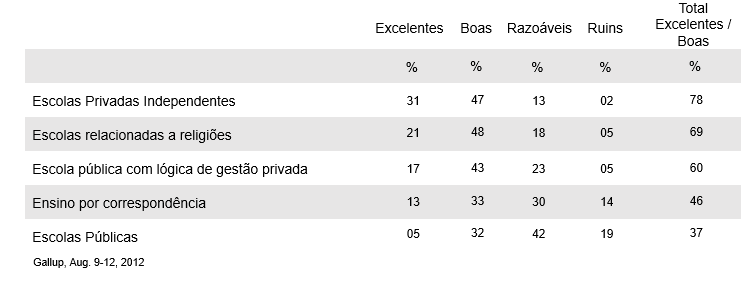
\includegraphics[width=0.8\textwidth]{3-4_binomial_distribution/homeschool.png}
\end{center}
}

\vspace{-30pt}
\soln{
{\footnotesize
\only<2->{
\begin{align*}
\mu &= np = 1,000 \times 0.13 = 130 \\
\sigma &= \sqrt{np(1-p)} = \sqrt{1,000 \times 0.13 \times 0.87} \approx 10.6
\end{align*}
}}}
\vspace{-10pt}
\begin{changemargin}{+1cm}{+0cm}
\pause
\begin{enumerate}
\justifying
\only<3->{\item[Método 1:] Intervalo de observações usuais:\\ $130 \pm 2 \times 10.6 = (108.8, 151.2)$ \\
\justifying
100 está fora desse intervalo, portanto, seria considerado incomum.}
\justifying
\only<4->{\item[Método 2:] Z-score de observação:\\ $Z = \frac{x - mean}{SD} = \frac{100 - 130}{10.6} = -2.83$ \\
100 é mais do que 2 SD abaixo da média, portanto, seria considerado incomum.}
\end{enumerate}
\end{changemargin}

\vfill
\justifying
\ct{\webURL{http://www.gallup.com/poll/156974/private-schools-top-marks-educating-children.aspx}}

\end{frame}
%%%%%%%%%%%%%%%%%%%%%%%%%%%%%%%%%%%

\subsection{Aproximação normal ao binômio}

%%%%%%%%%%%%%%%%%%%%%%%%%%%%%%%%%%%%

\begin{frame}
\frametitle{Formatos de distribuições binomiais}
\justifying
\app{Formatos de distribuições binomiais}
{
\justifying
Para esta atividade, você usará um applet da web. Vá para \webURL{https://gallery.shinyapps.io/dist_calc/} e escolha \textit{Binomial coin experiment} no menu suspenso à esquerda.
\begin{itemize}
\justifying
\item Defina o número de tentativas para 20 e a probabilidade de sucesso para 0,15. Descreva a forma da distribuição do número de sucessos.
\justifying
\item Mantendo $ p $ constante em 0,15, determine o tamanho mínimo de amostra necessário para obter uma distribuição unimodal e simétrica do número de sucessos.
\end{itemize}
}

\end{frame}
%%%%%%%%%%%%%%%%%%%%%%%%%%%%%%%%%%%%

\begin{frame}
\frametitle{Formatos de distribuições binomiais}
\begin{itemize}
\justifying
\item Outras considerações:
\begin{itemize}
\justifying
\item O que acontece com o formato da distribuição quando $ n $ permanece constante e $ p $ muda?
\justifying
\item O que acontece com o formato da distribuição quando $ p $ permanece constante e $ n $ muda?
\end{itemize}
\end{itemize}


\end{frame}

%%%%%%%%%%%%%%%%%%%%%%%%%%%%%%%%%%%%

\begin{frame}
\frametitle{Distribuições do número de sucessos}
\justifying
\dq{Histogramas de amostras do modelo binomial em que $ p = 0,10 $ e $ n = 10 $, $ 30 $, $ 100 $ e $ 300 $. O que acontece quando $ n $ aumenta?}

\begin{center}
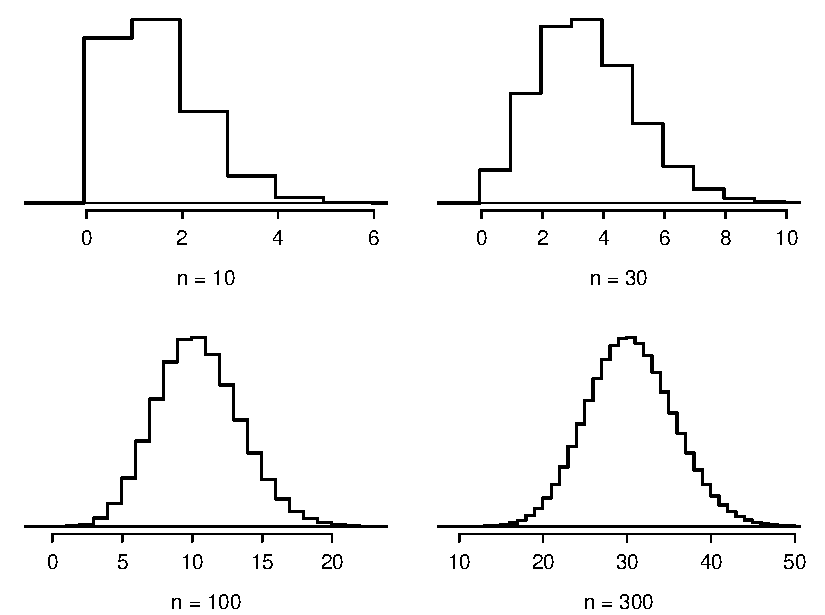
\includegraphics[width=0.60\textwidth]{3-4_binomial_distribution/fourBinomialModelsShowingApproxToNormal.pdf}
\end{center}

\end{frame}

%%%%%%%%%%%%%%%%%%%%%%%%%%%%%%%%%%%

\begin{frame}
\frametitle{Baixo grande é grande o suficiente?}
\justifying
O tamanho da amostra é considerado grande o suficiente se o número esperado de sucessos e fracassos forem pelo menos 10.
\[ np \ge 10 \qquad \text{ e } \qquad n(1-p) \ge 10 \]

\soln{\only<2->{$10 \times 0.13 = 1.3; 10 \times (1 - 0.13) = 8.7$}}

\end{frame}

%%%%%%%%%%%%%%%%%%%%%%%%%%%%%%%%%%

\begin{frame}
\frametitle{Prática}
\justifying
\pq{Abaixo estão quatro pares de parâmetros de distribuição binomial. Qual distribuição pode ser aproximada pela distribuição normal?}

\begin{enumerate}[(a)]
\item $n = 100, p = 0.95$
\solnMult{$n = 25, p = 0.45$} \soln{\only<2>{\orange{$\rightarrow 25 \times 0.45 = 11.25; 25 \times 0.55 = 13.75$}}}
\item $n = 150, p = 0.05$
\item $n = 500, p = 0.015$
\end{enumerate}

\end{frame}


%%%%%%%%%%%%%%%%%%%%%%%%%%%%%%%%%%%%

\begin{frame}
\frametitle{Uma análise dos usuários do Facebook}
\justifying
\dq{Um estudo recente descobriu que "os usuários do Facebook recebem mais do que dão". Por exemplo:
\begin{itemize}
\justifying
\item 40\% dos usuários do Facebook em nossa amostra fizeram uma solicitação de amizade, mas 63\% receberam pelo menos uma solicitação de amizade.
\justifying
\item Os usuários em nossa amostra deram like para o conteúdo dos seus amigos em média 14 vezes, mas tiveram seu conteúdo "curtido" em média 20 vezes.
\justifying
\item Os usuários enviaram 9 mensagens pessoais, mas receberam 12.

\end{itemize}
}
\end{frame}
%%%%%%%%%%%%%%%%%%%%%%%%%%%%%%%%%%%%

\begin{frame}
\frametitle{Uma análise dos usuários do Facebook}
\begin{itemize}
\justifying
\item 12\% dos usuários marcaram um amigo em uma foto, mas 35\% foram marcados em uma foto.
\end{itemize}
\justifying
\hl{Algum palpite de como esse padrão pode ser explicado?}

\justifying
\soln{\only<2>{Usuários ativos contribuem com muito mais conteúdo do que o usuário padrão.}}
\justifying
\ct{\webURL{http://www.pewinternet.org/Reports/2012/Facebook-users/Summary.aspx}}

\end{frame}

%%%%%%%%%%%%%%%%%%%%%%%%%%%%%%%%%%%

\begin{frame}
\frametitle{Prática}
\justifying
\dq{Este estudo também descobriu que aproximadamente 25\% dos usuários do Facebook são considerados usuários ativos. O mesmo estudo descobriu que o usuário médio do Facebook tem 245 amigos. Qual é a probabilidade de que o usuário médio do Facebook com 245 amigos tenha 70 ou mais amigos que seriam considerados usuários ativos? Anote todas as suposições que você fizer.}
\justifying
Temos que $ n = 245, p = 0.25 $ e queremos saber a probabilidade $ P (K \ge 70) $. Para prosseguir, precisamos de independência, o que vamos assumir, mas podemos tentar obter mais dados do Facebook.

\pause
\end{frame}
%%%%%%%%%%%%%%%%%%%%%%%%%%%%%%%%%%%

\begin{frame}
\frametitle{Prática}
\begin{align*}
P(X \ge 70) &= P(K = 70\text{ ou }K = 71\text{ ou }K = 72\text{ ou }\cdots\text{ ou } K = 245) \\
&= P(K = 70) + P(K = 71) + P(K = 72) + \cdots + P(K = 245)
\end{align*}

\pause
\justifying
Isso parece um monte de trabalho ...

\end{frame}

%%%%%%%%%%%%%%%%%%%%%%%%%%%%%%%%%%%%

\begin{frame}
\frametitle{Aproximação normal ao binômio}
\justifying
Quando o tamanho da amostra é grande o suficiente, a distribuição binomial de parâmetros $ n $ e $ p $ pode ser aproximada pelo modelo normal com os parâmetros $ \mu = np $ e $ \sigma = \sqrt {np (1-p)} $.

\begin{itemize}
\justifying
\item No caso dos usuários avançados do Facebook, $n = 245$ e $p = 0.25$.
\[ \mu = 245 \times 0.25 = 61.25 \qquad \sigma = \sqrt{245 \times 0.25 \times 0.75} = 6.78 \]
\justifying
\item $Bin(n = 245, p = 0.25) \approx N(\mu = 61.25, \sigma = 6.78)$.

\begin{center}
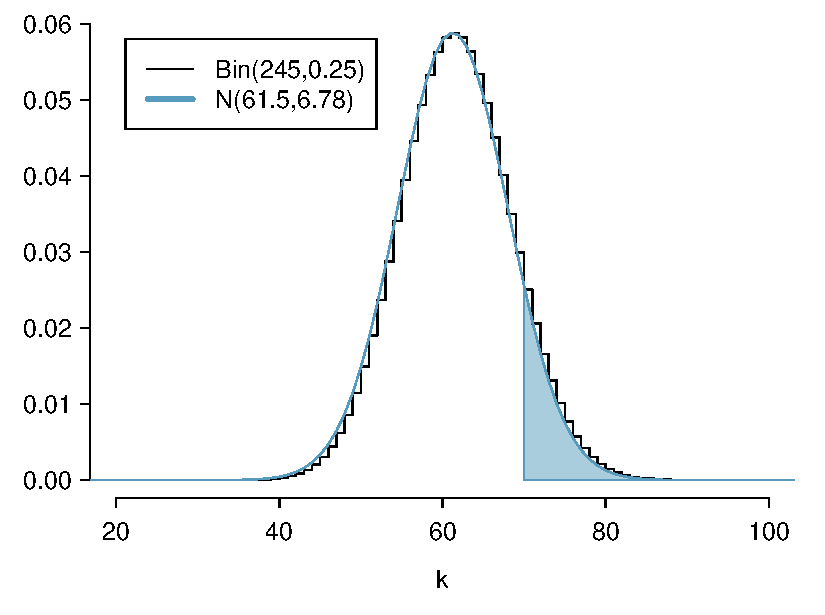
\includegraphics[width=0.4\textwidth]{3-4_binomial_distribution/fb_power_user.pdf}
\end{center}

\end{itemize}

\end{frame}

%%%%%%%%%%%%%%%%%%%%%%%%%%%%%%%%%%%

\begin{frame}
\frametitle{Prática}
\justifying
\dq{Qual é a probabilidade de o usuário médio do Facebook com 245 amigos ter 70 ou mais amigos que seriam considerados usuários avançados?}

\pause

\twocol{0.4}{0.6}{
\begin{center}
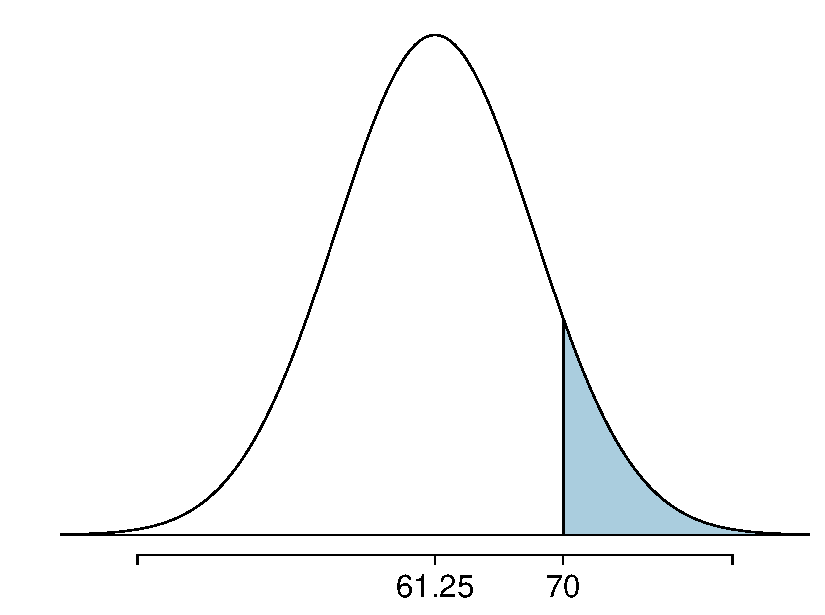
\includegraphics[width=\textwidth]{3-4_binomial_distribution/fb_power_user_norm.pdf}
\end{center}
}
{
\pause
\[ Z = \frac{obs - \textit{média}}{SD} = \frac{70 - 61.25}{6.78} = 1.29 \]

\pause
{\footnotesize
\begin{tabular}{c | rrrr>{\columncolor[gray]{0.6}[0pt]}r |}
  \cline{2-6}
& \multicolumn{5}{c}{Segunda casa decimal de $Z$}  \\
  \cline{2-6}
$Z$ & 0.05 & 0.06 & 0.07 & 0.08 & 0.09   \\
  \hline
  \hline
  1.0 & \tiny{0.8531} & \tiny{0.8554} & \tiny{0.8577} & \tiny{0.8599} & \tiny{0.8621} \\
  1.1 & \tiny{0.8749} & \tiny{0.8770} & \tiny{0.8790} & \tiny{0.8810} & \tiny{0.8830} \\
\rowcolor[gray]{.6}
  1.2 & \tiny{0.8944} & \tiny{0.8962} & \tiny{0.8980} & \tiny{0.8997} & \orange{\tiny{0.9015}} \\  
\end{tabular}
}

\pause
\[ P(Z > 1.29) = 1 - 0.9015 = 0.0985 \]
}

\end{frame}

%%%%%%%%%%%%%%%%%%%%%%%%%%%%%%%%%%

